\documentclass[10pt]{beamer}

\usepackage{polyglossia}
\usepackage{csquotes}
\usepackage{datetime}
\usepackage{fontspec}
\usepackage{microtype}
\usepackage{color}
\usepackage{url}
\usepackage{hyperref}
\usepackage{amsfonts}
\usepackage{amsmath}
\usepackage{amsthm}
\usepackage{subcaption}
\usepackage[backend=biber,style=iso-authoryear,sortlocale=en_US,autolang=other,bibencoding=UTF8]{biblatex}
\usepackage{booktabs}
\usepackage{graphics}
\usepackage{pifont}
\usepackage{tikz}

\addbibresource{zotero.bib}

\setdefaultlanguage{english}
\usefonttheme{professionalfonts}
\setmainfont{TeX Gyre Termes}
\usetheme{Boadilla}
\usecolortheme{crane}
\setbeamertemplate{title page}[default][rounded=true,shadow=false]
\setbeamertemplate{section in toc}[ball unnumbered]
\setbeamertemplate{bibliography item}{}

\hypersetup{
	pdfencoding=auto,
	unicode=true,
	citecolor=green,
	filecolor=blue,
	linkcolor=red,
	urlcolor=blue
}

\makeatletter
\newcommand*{\currentSection}{\@currentlabelname}
\makeatother

\title[Graph neural networks]
{
	Graph neural networks
}

\date[2024-04-04]{4 April 2024}

\author[Marek Dědič]
{
	Marek~Dědič
}

\AtBeginSection[]{
	\begin{frame}{\currentSection}
		\tableofcontents[currentsection]
	\end{frame}
}

\newcommand{\mathvec}{\ensuremath{\mathbf}}
\newcommand{\mathmat}{\ensuremath{\mathbf}}
\newcommand{\mathspace}{\ensuremath{\mathcal}}
\newcommand{\mathfield}{\ensuremath{\mathbb}}

\begin{document}

\begin{frame}
	\titlepage
\end{frame}

\begin{frame}{Outline}
	\tableofcontents
\end{frame}

% Body

\section{Motivation}

\begin{frame}{Motivation}
	\begin{itemize}
		\item Graphs are a natural way of abstracting many mathematical and real-world problems
		\item Use in chemistry, software engineering, image recognition, medicine, particle physics, network security, fake-news detection, autonomous vehicles etc.
	\end{itemize}
	\centering
	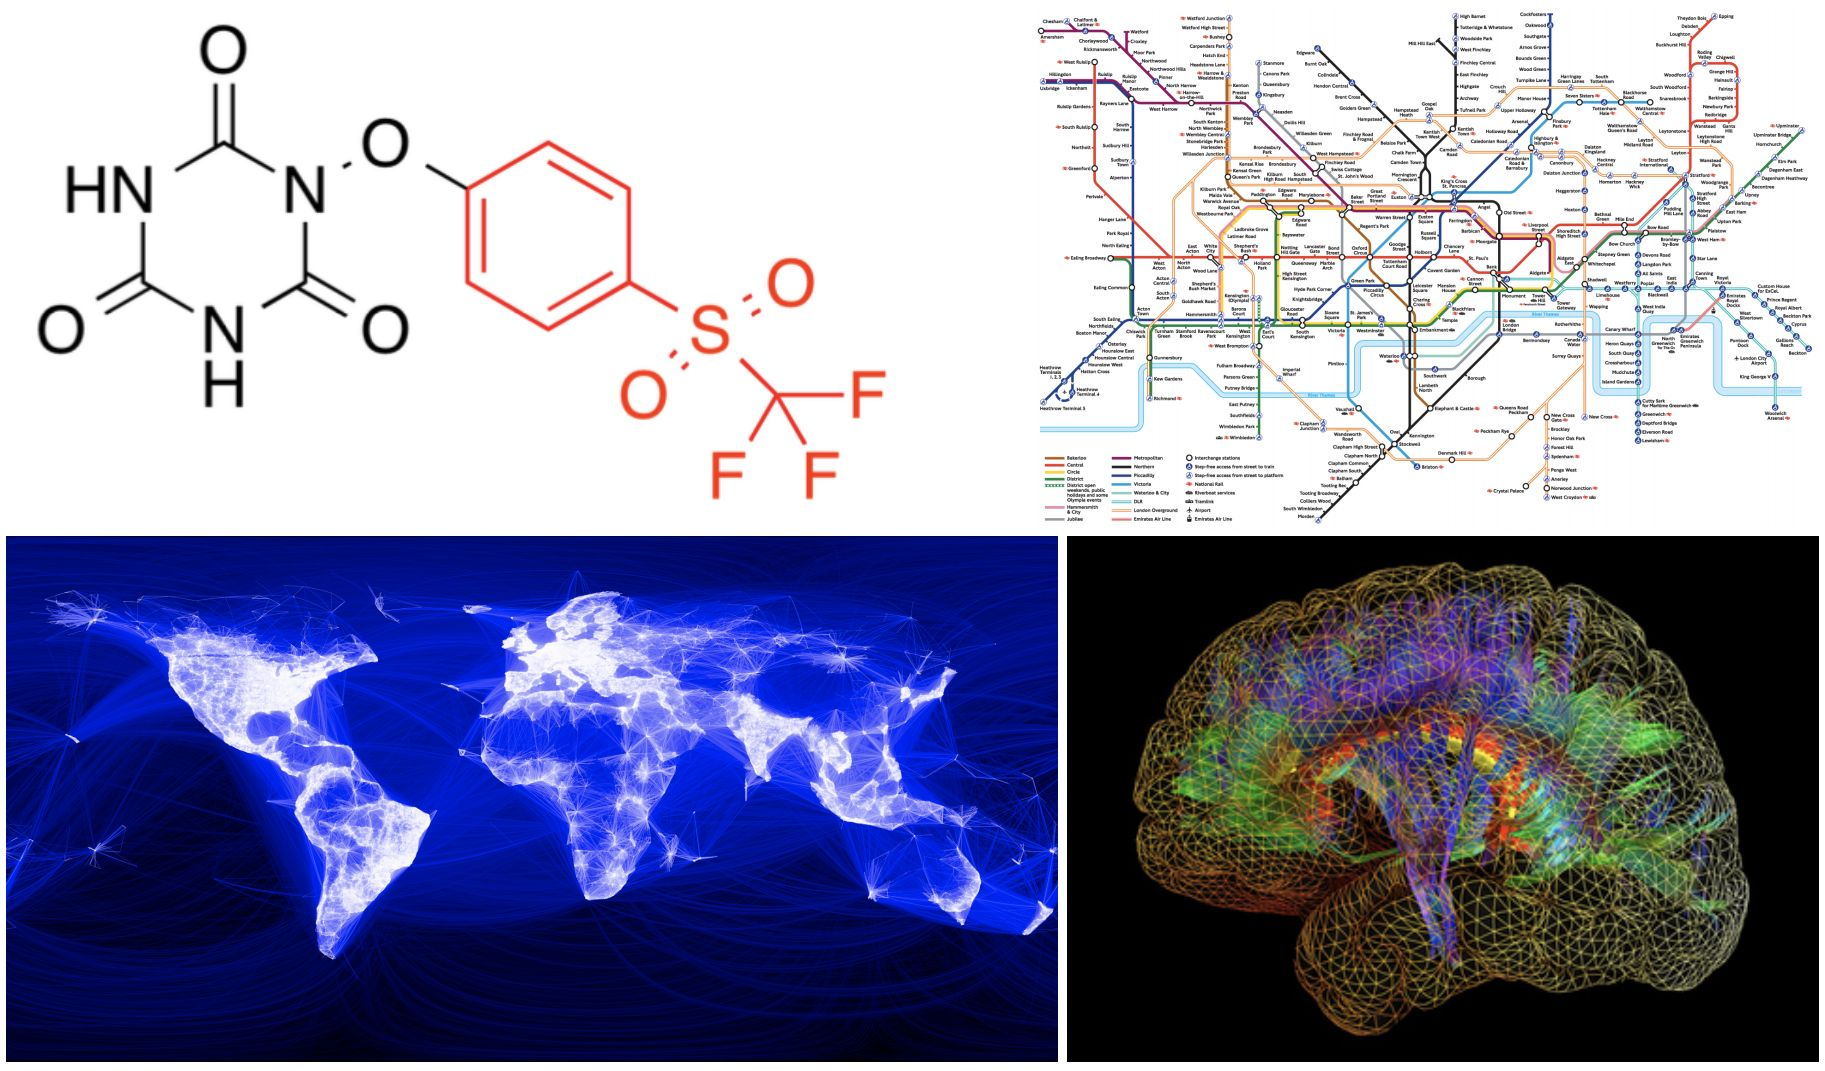
\includegraphics[width=0.7\pagewidth]{images/graphs.png}\footnote{\cite{velickovic_opening_2020}}
\end{frame}

\begin{frame}{Basic definitions}
	\begin{itemize}
		\item Graph \( G = \left( V, E \right) \)
		\item \( ne \left[ v \right] \) is the set of nodes connected to \( v \) by an edge.
		\item \( co \left[ v \right] \) is the set of edges incident on (i.e. containing) \( v \).
		\item \( x_v \) are the features of node \( v \).
		\item \( x_e \) are the features of edge \( e \).
	\end{itemize}
\end{frame}

\section{Tasks on graphs}

\begin{frame}{Node classification}
	\centering
	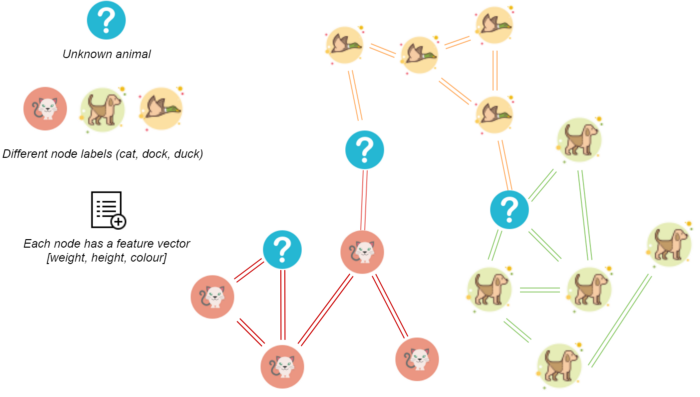
\includegraphics[width=0.7\pagewidth]{images/node-classification.png}\footnote{\cite{kubara_machine_2020}}
\end{frame}

\begin{frame}{Link prediction}
	\centering
	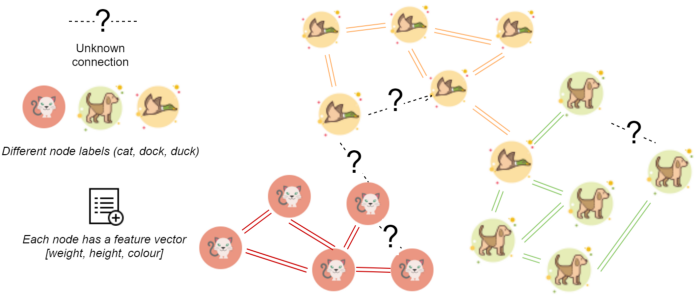
\includegraphics[width=0.7\pagewidth]{images/link-prediction.png}\footnote{\cite{kubara_machine_2020}}
\end{frame}

\begin{frame}{Graph classification}
	\centering
	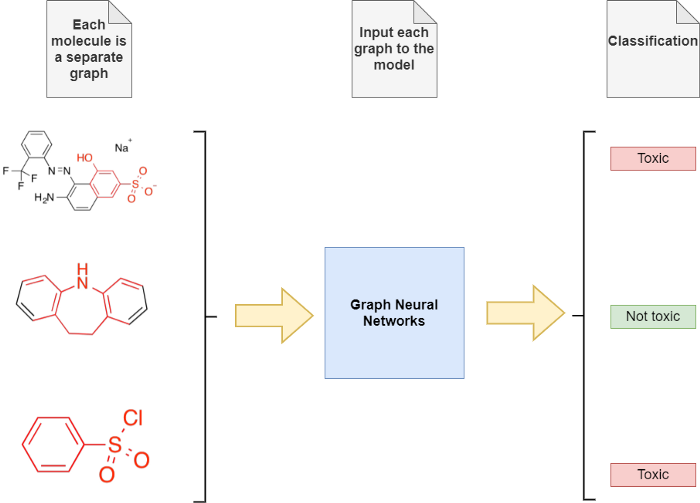
\includegraphics[width=0.7\pagewidth]{images/whole-graph-learning.png}\footnote{\cite{kubara_machine_2020}}
\end{frame}

\begin{frame}{Community detection}
	\centering
	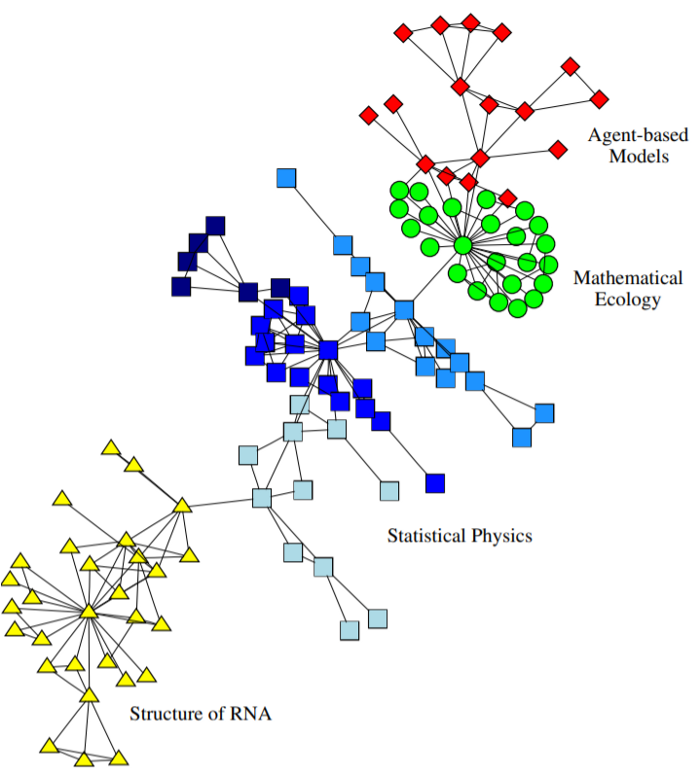
\includegraphics[width=0.5\pagewidth]{images/community-detection.png}\footnote{\cite{girvan_community_2002}}
\end{frame}

\section{GNN}

\begin{frame}{GNN 1}
	\begin{itemize}
		\item We are solving \enquote{Node classification}.
		\item Adpating regular neural networks to graph data
		\item Formally defined as classification on the space \( \mathspace{G} \times \mathspace{N} \) -- pairs of a graph and one of its nodes
		\item We assume that for each node \( v \) and edge \( e \) we have features \( \mathvec{x}_v \) and \( \mathvec{x}_e \).
		\item For each node \( v \) we model a hidden state \( \mathvec{h}_v \) capturing information about \( v \) and its neighbourhood
	\end{itemize}
\end{frame}

\begin{frame}{GNN 2}
	\begin{itemize}
		\item For each node \( v \) we model a hidden state \( \mathvec{h}_v \) capturing information about \( v \) and its neighbourhood as
			\[ \mathvec{h}_v = f \left( \mathvec{x}_v, \mathvec{x}_{co \left[ v \right]}, \mathvec{h}_{ne \left[ v \right]}, \mathvec{x}_{ne \left[ v \right]} \right) \]
		\item ...and the output for \( v \) as
			\[ \mathvec{o}_v = g \left( \mathvec{h}_v, \mathvec{x}_v \right) \]
		\item We can compute the hidden states \( \mathvec{h}_v \) for all nodes together iteratively as
			\[ \mathmat{H}^{t + 1} = F \left( \mathmat{H}^t, \mathmat{X} \right) \]
	\end{itemize}
\end{frame}

\begin{frame}{GNN 3}
	\centering
	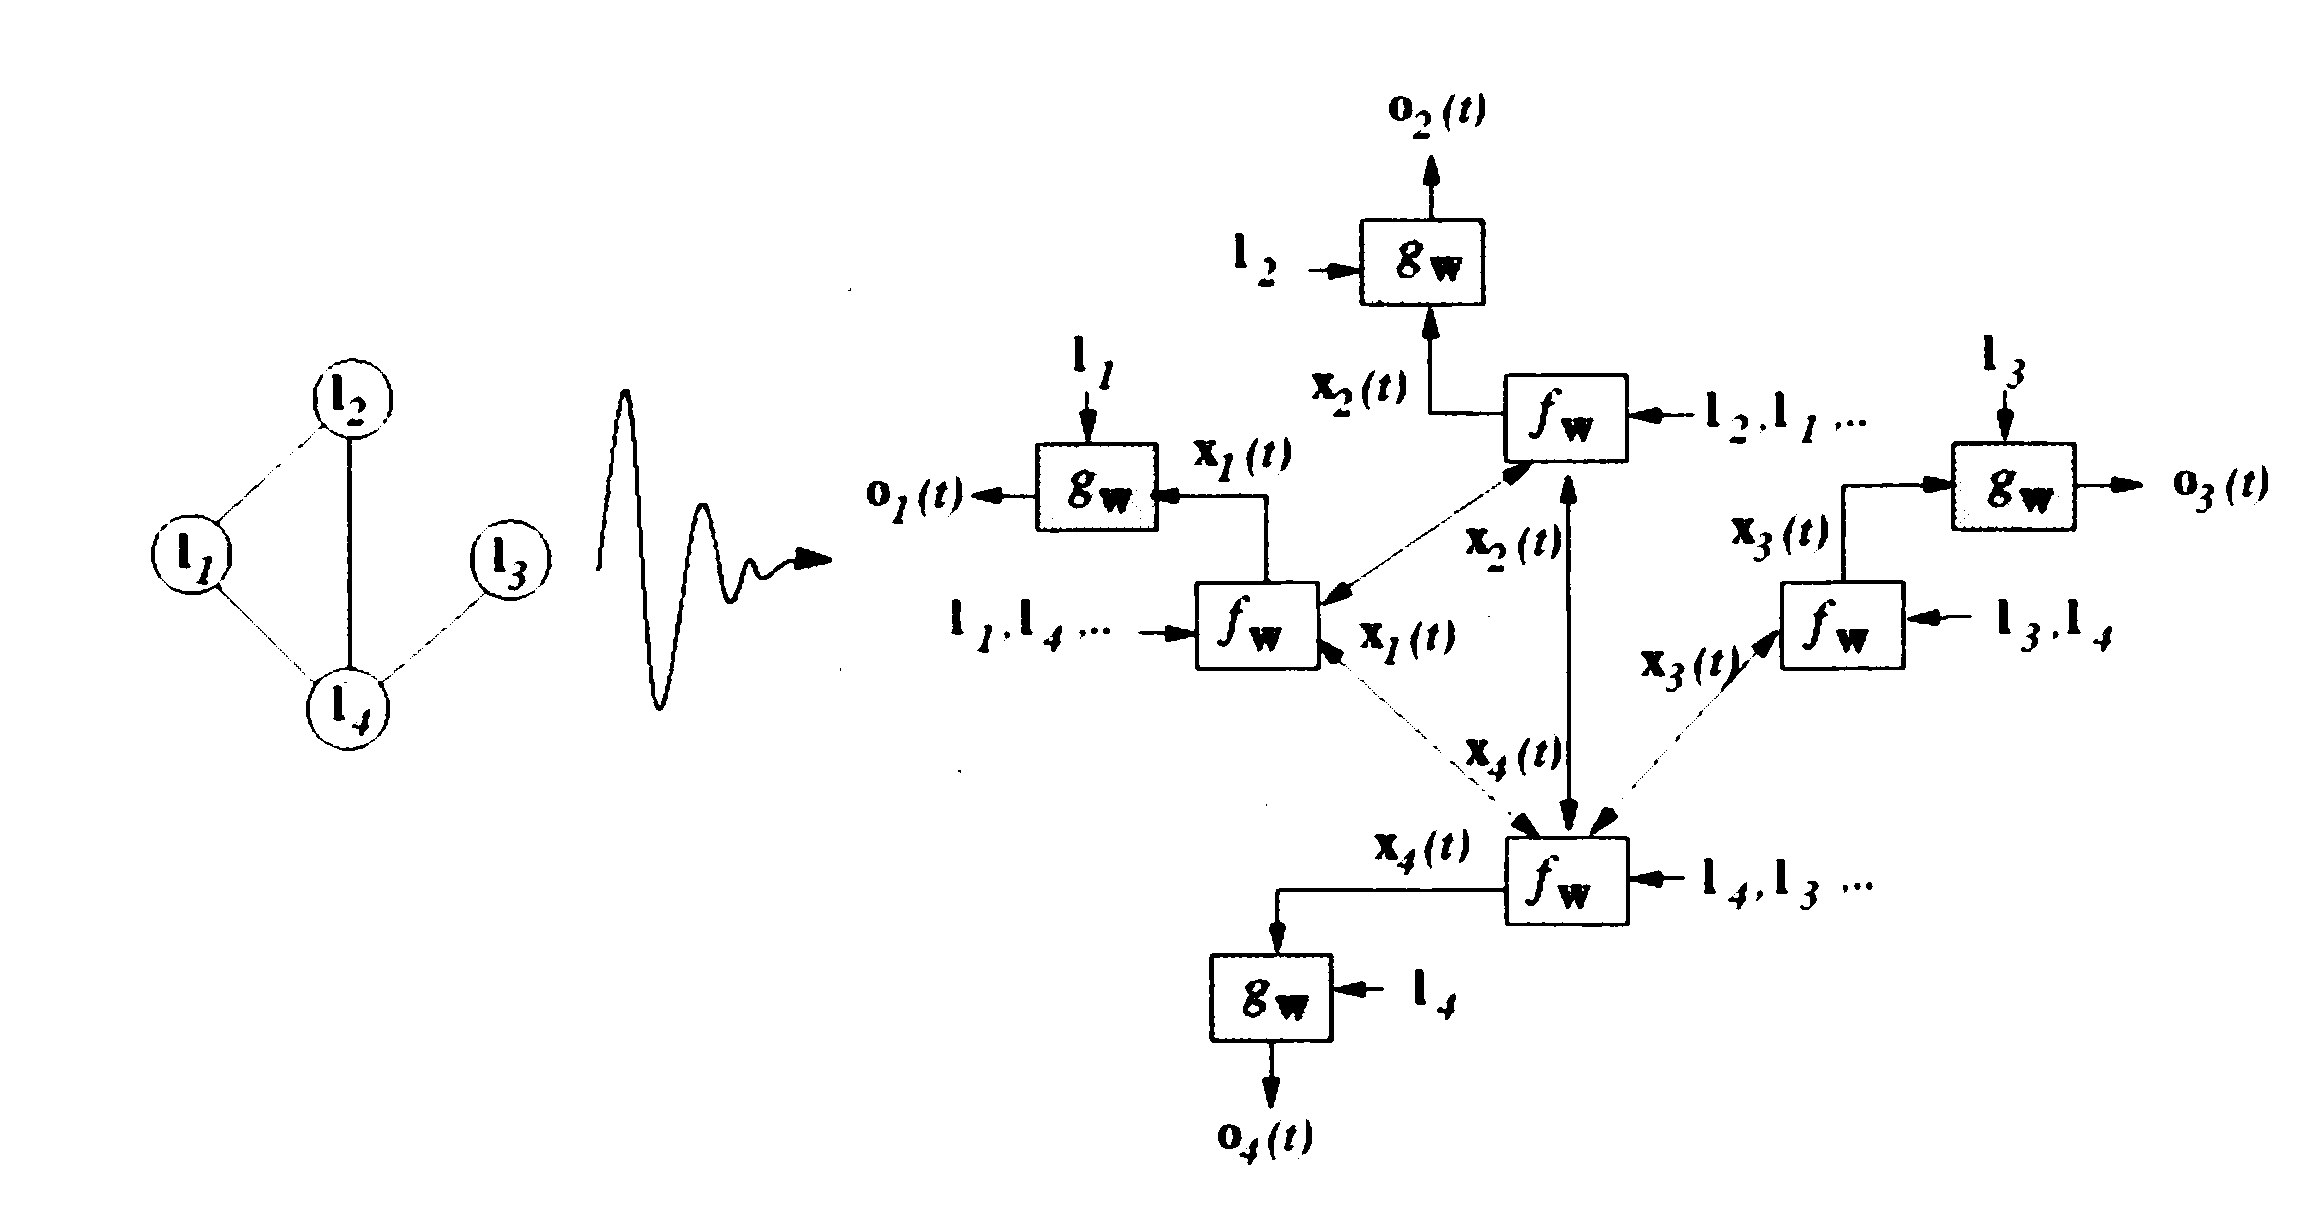
\includegraphics[width=0.9\pagewidth]{images/GNN.png}\footnote{\cite{gori_new_2005}}
\end{frame}

\begin{frame}{GNN -- conclusion}
	\begin{itemize}
		\item The iterative application of \( F \) can be understood as an instance of a RNN.
		\item This iterative process can be unrolled into a regular MLP.
		\item There are no hidden states for edges, only nodes.
	\end{itemize}
\end{frame}

\begin{frame}{GNN -- modifications}
	\begin{figure}[h]
		\centering
		\begin{subfigure}[t]{0.33\textwidth}
			\centering
			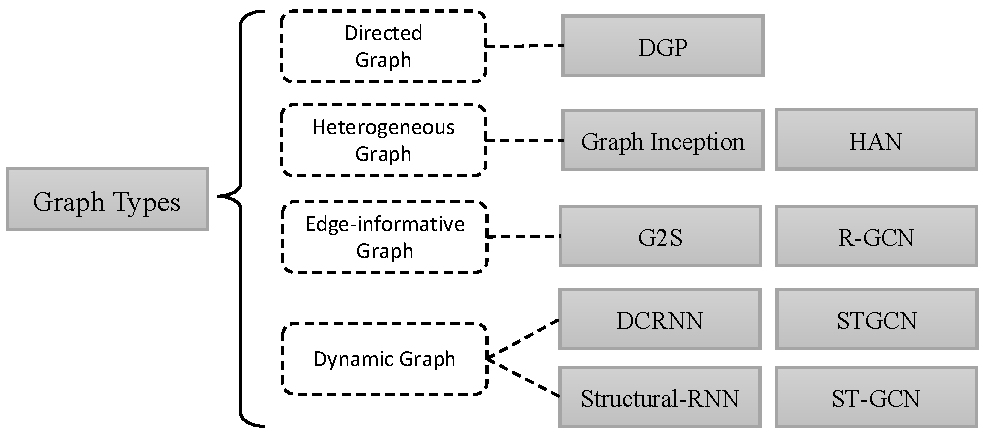
\includegraphics[width=1\linewidth]{images/GNN-variants/variant1.pdf}
		\end{subfigure}
		\begin{subfigure}[t]{0.43\textwidth}
			\centering
			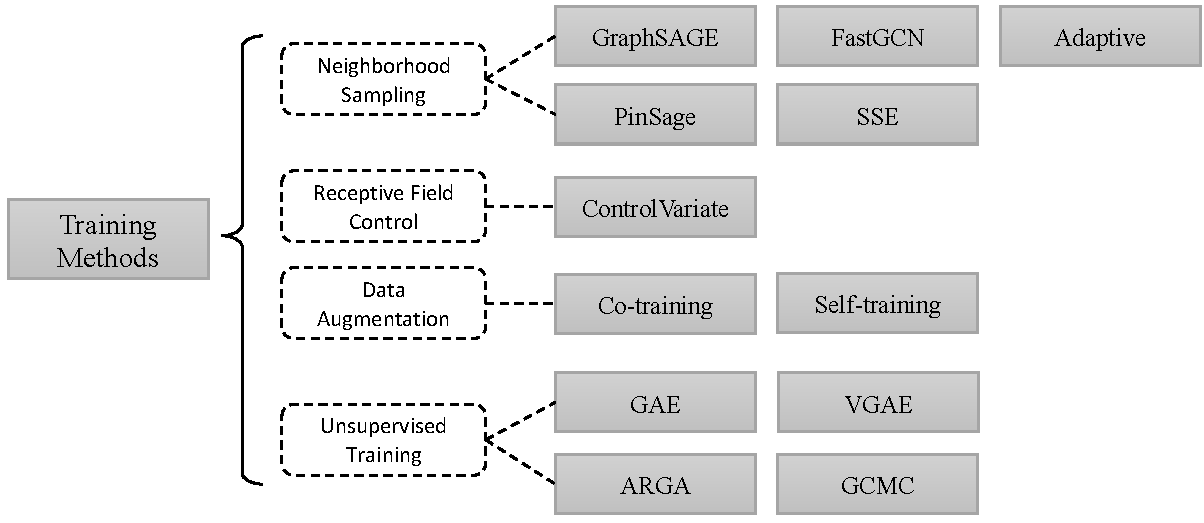
\includegraphics[width=1\linewidth]{images/GNN-variants/variant3.pdf}
		\end{subfigure}
		\begin{subfigure}[t]{0.65\textwidth}
			\centering
			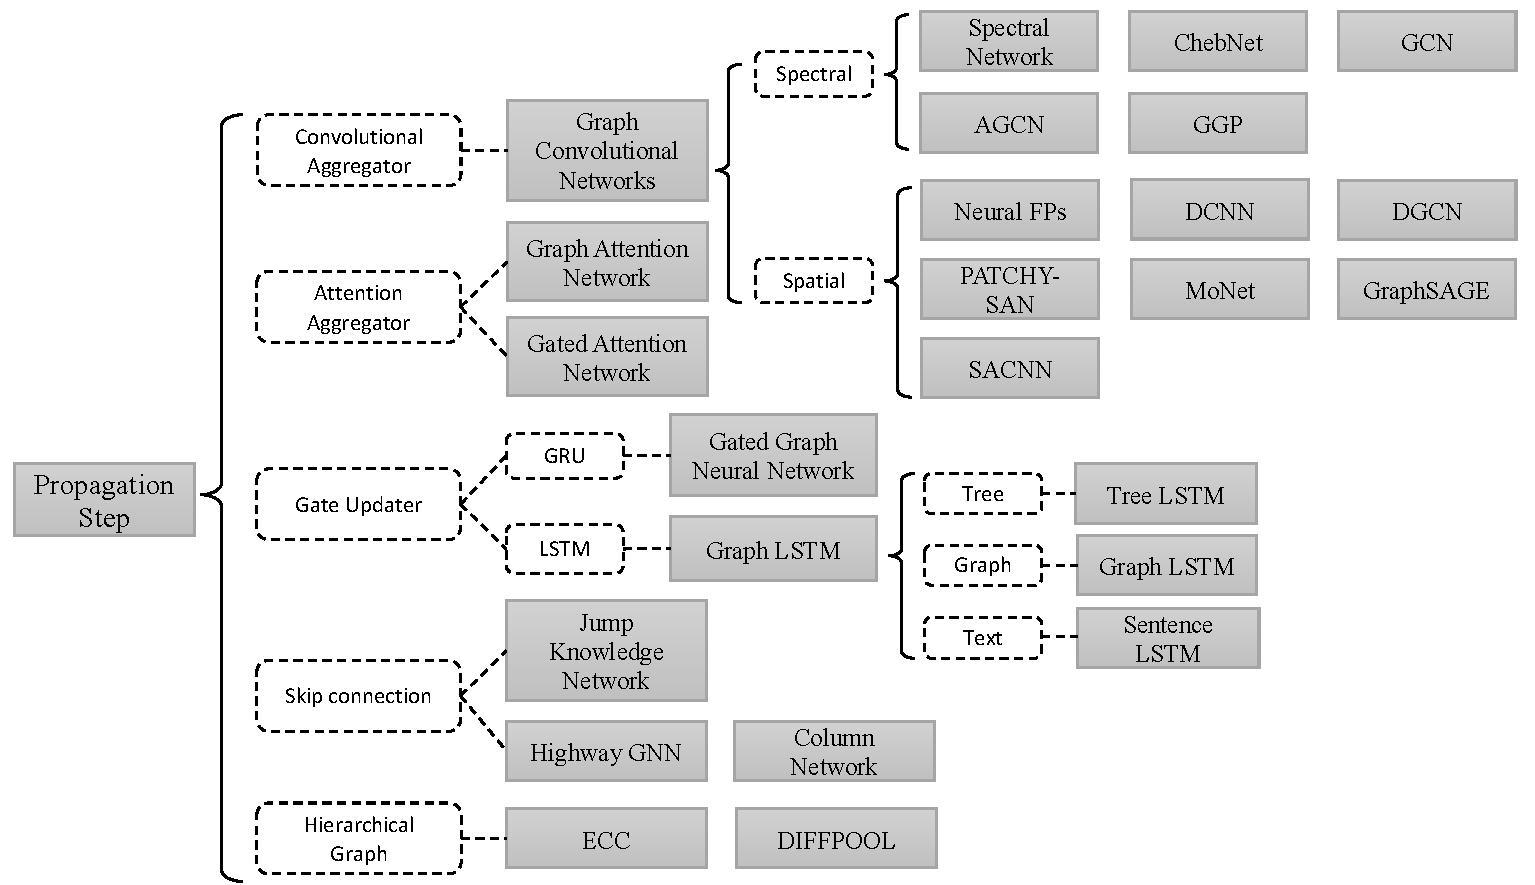
\includegraphics[width=1\linewidth]{images/GNN-variants/variant2.pdf}
		\end{subfigure}
	\end{figure}\footnote{\cite{zhou_graph_2019}}
\end{frame}

\section{DeepWalk}

\begin{frame}{DeepWalk 1}
	\begin{itemize}
		\item Inspired by word2vec and skip-gram -- techniques used for NLP
		\item Random walks from a given node (\( M \) walks of length \( L \))
	\end{itemize}
\end{frame}

\begin{frame}{DeepWalk 2}
	\centering
	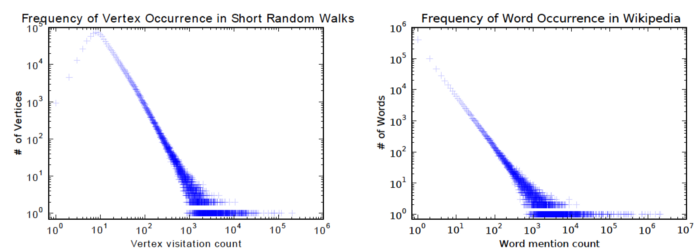
\includegraphics[width=0.8\pagewidth]{images/DeepWalk-word2vec.png}\footnote{\cite{perozzi_deepwalk_2014}}
\end{frame}

\begin{frame}{DeepWalk -- skip-gram}
	\centering
	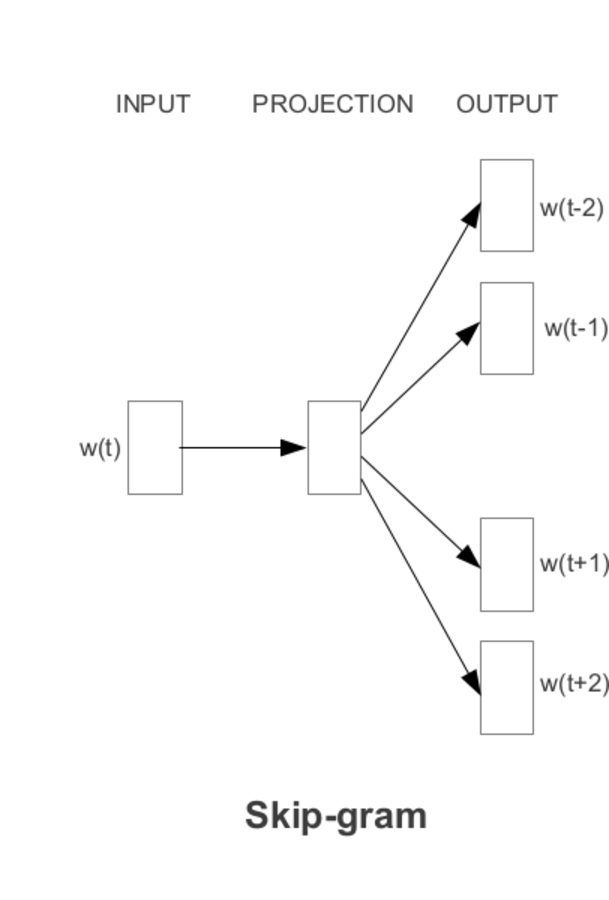
\includegraphics[width=0.4\pagewidth]{images/SkipGram.pdf}\footnote{\cite{mikolov_efficient_2013}}
\end{frame}

\begin{frame}{DeepWalk 4}
	\begin{itemize}
		\item For each node \( v \) we learn its representation \( f : \mathspace{V} \to \mathfield{R}^{\left\lvert \mathfield{V} \right\rvert \times d} \)
		\item We maximize the value of
			\[ \mathrm{P} \left( \left\{ v_{i - w}, \dots, v_{i + w} \right\} \setminus v_i \middle| f \left( v_i \right) \right) \]
		\item Assuming independence, this can be simplified to
			\[ \mathrm{P} \left( \left\{ v_{i - w}, \dots, v_{i + w} \right\} \setminus v_i \middle| f \left( v_i \right) \right) = \prod_{\substack{j = i - w \\ j \neq i}}^{i + w} \mathrm{P} \left( v_j \middle| f \left( v_i \right) \right) \]
		\item This is a problem word2vec can solve.
		\item There are further optimisations such as using a hierarchical softmax function
	\end{itemize}
\end{frame}

\begin{frame}{DeepWalk -- conclusion}
	\begin{itemize}
		\item Adapting the main ideas of word2vec to learn on graphs
		\item There is no way to classify new nodes -- the model needs to be retrained.
	\end{itemize}
\end{frame}

\section{node2vec}

\begin{frame}{node2vec 1}
	\begin{itemize}
		\item Also inspired by word2vec, albeit in a different way
		\item We are looking for the embedding \( \mathrm{node2vec} : \mathspace{G} \to \mathfield{R}^n \).
	\end{itemize}
\end{frame}

\begin{frame}{node2vec 2}
	\centering
	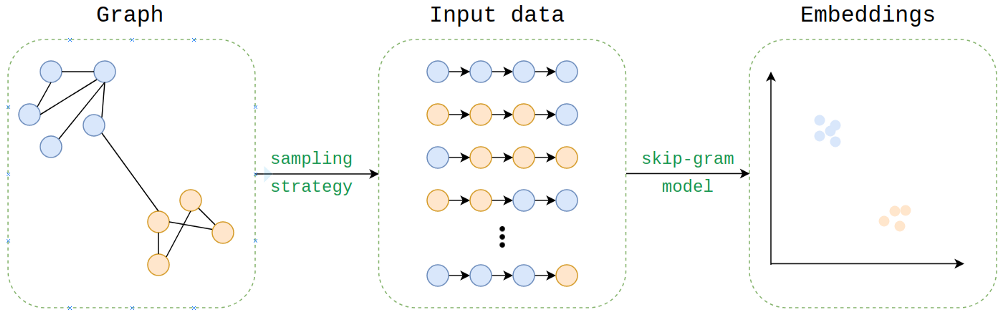
\includegraphics[width=0.9\pagewidth]{images/node2vec.png}\footnote{\cite{cohen_node2vec_2018}}
\end{frame}

\begin{frame}{node2vec 3}
	\begin{itemize}
		\item For each node \( v \) we learn its representation \( f : \mathspace{V} \to \mathfield{R}^{\left\lvert \mathfield{V} \right\rvert \times d} \)
		\item We maximize the value of
			\[ \mathrm{P} \left( ne \left[ v \right] \middle| f \left( v \right) \right) \]
		\item Assuming independence, this can be simplified to
			\[ \mathrm{P} \left( ne \left[ v \right] \middle| f \left( v \right) \right) = \prod_{v_i \in ne \left[ v \right]} \mathrm{P} \left( v_i \middle| f \left( v \right) \right) \]
		\item There are further optimisations such as using a hierarchical softmax function and negative sampling
	\end{itemize}
\end{frame}

\begin{frame}{node2vec 4}
	\begin{itemize}
		\item How to explore \( ne \left[ v \right] \)?
		\item 2 extremes: BFS, DFS
		\item Regular random walk: When I am in the node \( v \), I continue to any node adjacent to \( v \), with the same probability for all neighbours.
		\item Let's modify random walks to interpolate between BFS and DFS
		\item When arriving from node \( t \) to node \( v \) and choosing where to go next, we assign to each neighbour \( x \) a weight
			\[ \alpha \left( t, x \right) = \begin{cases}
				\frac{1}{p} &\text{ pro } d_{tx} = 0 \\
				1 &\text{ pro } d_{tx} = 1 \\
				\frac{1}{q} &\text{ pro } d_{tx} = 2 \\
			\end{cases} \]
			where \( d_{tx} \) is the shortest path distance from \( t \) to \( x \) and \( p, q \) are parameters.
	\end{itemize}
\end{frame}

\begin{frame}{node2vec 5}
	\centering
	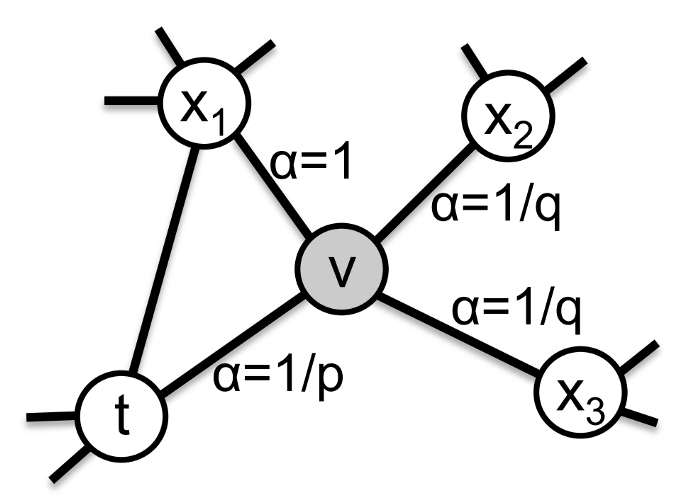
\includegraphics[width=0.7\pagewidth]{images/node2vec-alpha.png}\footnote{\cite{grover_node2vec_2016}}
\end{frame}

\begin{frame}{node2vec -- conclusion}
	\begin{itemize}
		\item Adapting the main ideas of word2vec to learn on graphs
		\item Improving on DeepWalk
		\item There is no way to classify new nodes -- the model needs to be retrained.
	\end{itemize}
\end{frame}

\begin{frame}{node2vec -- demo}
\end{frame}

\section{GCN}

\begin{frame}{GCN 1}
	\begin{itemize}
		\item We are solving \enquote{Node classification}.
		\item GCN is inspired by convolutional networks
	\end{itemize}
\end{frame}

\begin{frame}{GCN 2}
	\begin{itemize}
		\item We express the neural network as operating on the whole graph, similarily to the basic GNN
		\item Each layer is of the form
			\[ \mathmat{H}^{l + 1} = f \left( \mathmat{H}^{(l)}, \mathmat{A} \right) \]
			where \( \mathmat{A} \) is the adjacency matrix of the graph.
		\item A simple layer can be implemented as
			\[ f \left( \mathmat{H}^{(l)}, \mathmat{A} \right) = \sigma \left( \mathmat{A} \mathmat{H}^{(l)} \mathmat{W}^{(l)} \right) \]
			where \( \mathmat{W} \) are weights and \( \sigma \) the activation function.
	\end{itemize}
\end{frame}

\begin{frame}{GCN 3}
	\begin{itemize}
		\item Using \( \mathmat{A} \), we would forget information in the current node in each step. To solve this, we replace \( \mathmat{A} \) with \( \widehat{\mathmat{A}} = \mathmat{A} + \mathmat{I} \).
		\item Because \( \mathmat{A} \) isn't normalized, the output of each layer would have a different magnitude, leading to computational instability. To prevent that, we replace \( \mathmat{A} \) with its symmetrically normalized variant \( \mathmat{D}^{-\frac{1}{2}} \mathmat{A} \mathmat{D}^{-\frac{1}{2}} \), whete \( \mathmat{D} \) is the diagonal matrix of node degrees.
		\item This gives us one layer of GCN as
			\[ f \left( \mathmat{H}^{(l)}, \mathmat{A} \right) = \sigma \left( \widehat{\mathmat{D}}^{-\frac{1}{2}} \widehat{\mathmat{A}} \widehat{\mathmat{D}}^{-\frac{1}{2}} \mathmat{H}^{(l)} \mathmat{W}^{(l)} \right) \]
	\end{itemize}
\end{frame}

\begin{frame}{GCN 4}
	\centering
	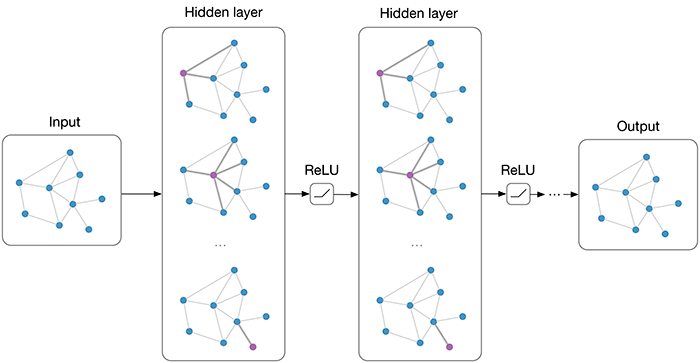
\includegraphics[width=0.8\pagewidth]{images/GCN.png}\footnote{\cite{kipf_how_2016}}
\end{frame}

\begin{frame}{GCN -- conclusion}
	\begin{itemize}
		\item Adapting the main ideas of CNNs to learn on graphs
		\item GCNs are a first-order approximation of local spectral filters on graphs -- see \cite{kipf_semi-supervised_2017}.
	\end{itemize}
\end{frame}

\section{GraphSAGE}

\begin{frame}{GraphSAGE 1}
	\begin{itemize}
		\item GraphSAGE is an inductive method -- it doesn't need the whole graph for training
		\item The representation of \( v \) is learned using its neighbours, i.e.
			\[ \mathvec{h}_v^{(l + 1)} = \sigma \left( \mathmat{W}^{(l)} \cdot \mathrm{concat} \left( \mathvec{h}_v^{(l)}, \mathvec{h}_{ne \left[ v \right]}^{(l)} \right) \right) \]
			where
			\[ \mathvec{h}_{ne \left[ v \right]}^{(l)} = \textsc{aggregate}_l \left( \left\{ \mathvec{h}_u^{(l)} \middle| u \in ne \left[ v \right] \right\} \right) \]
		\item We need a special loss function
	\end{itemize}
\end{frame}

\begin{frame}{GraphSAGE 2}
	\centering
	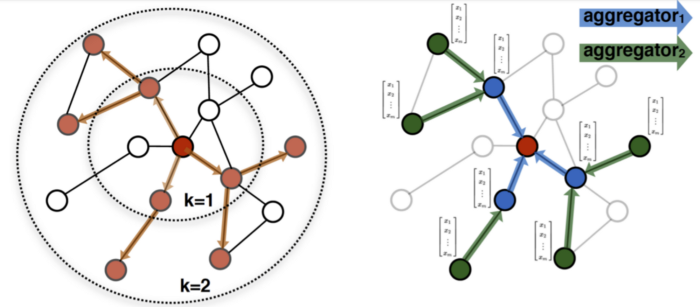
\includegraphics[width=0.7\pagewidth]{images/GraphSAGE.png}\footnote{\cite{hamilton_inductive_2017}}
\end{frame}

\begin{frame}{GraphSAGE 3}
	\begin{itemize}
		\item We can choose aggregators for each layer
		\item Arithmetic mean leads to GCN
		\item LSTM aggregator (with neighbour permutation)
		\item Pooling:
			\[ \textsc{aggregate}_l = \max \left\{ \sigma \left( \mathmat{W}_{\mathrm{pool}} \mathvec{h}_u^{(l)} + \mathvec{b} \right) \middle| u \in ne \left[ v \right] \right\} \]
	\end{itemize}
\end{frame}

\begin{frame}{GraphSAGE -- conclusion}
	\begin{itemize}
		\item The inductive approach is good for graphs where additional nodes may be added.
		\item The model will work (reasonably well) with new data points
	\end{itemize}
\end{frame}

\begin{frame}
	\centering
	
\includegraphics[width=0.75\pagewidth]{images/thats-all.png}
\end{frame}

\begin{frame}[allowframebreaks]{Read more}
	\printbibliography
\end{frame}

\end{document}
